\documentclass[a4paper,12pt,twoside]{report}

\usepackage{acronym}
\usepackage{url}
\usepackage{cite}
\usepackage{listings}
\usepackage[pdftex]{graphicx}
\usepackage[hang,small,bf]{caption}
\usepackage{styles/tum}
\usepackage{styles/usecases}
\usepackage{setspace}
\usepackage[german,english]{babel}
\usepackage{float}
\usepackage{floatflt}
\usepackage{fancyhdr}
\usepackage{color}
\usepackage{booktabs}
\usepackage[pdftex,bookmarks=true,plainpages=false,pdfpagelabels=true]{hyperref}
\usepackage{mdwlist}
\usepackage{enumerate}
\usepackage{paralist}
\usepackage{array}
\usepackage{longtable}
\usepackage{listings}
\usepackage[utf8]{inputenc}
\usepackage[capitalize, noabbrev]{cleveref}

% Path for graphics
\graphicspath{{figures/}}

\begin{document}
\setlength{\evensidemargin}{22pt}
\setlength{\oddsidemargin}{22pt}

\def\doctype{Master's Thesis}
\def\faculty{Informatik}
\def\title{Using Synthetic Data for Classification of Small Parts}		%TODO add title in German
\def\titleGer{Synthetische Daten für die Klassifizierung von Kleinteilen verwenden}	%TODO add title in German
\def\supervisor{Prof. Bernd Brügge, Ph.D.}
\def\advisor{Sajjad Taheri, M.Sc.}
\def\author{Amr Abdelraouf}
\def\date{15.10.2018}		%TODO add submission / handover date


\hypersetup{pdfborder={0 0 0},
                        pdfauthor={Amr Abdelraouf},
                        pdftitle={Using Synthetic Data for Classification of Small Parts},
                        }

\lstset{showspaces=false, numbers=left, frame=single, basicstyle=\small}

\pagenumbering{alph}

\thispagestyle{empty}

\vspace{4cm}
\begin{center}
\oTUM{4cm}\\ 
\vspace{5mm}     
\huge FAKULT{\"A}T F{\"U}R INFORMATIK\\ 
\vspace{0.5cm}
\large DER TECHNISCHEN UNIVERSIT{\"A}T M{\"U}NCHEN\\
\vspace{1mm}
\end{center}

\vspace{13mm}

\begin{center}
{\Large \doctype\ in \faculty}
\vspace{20mm}

\begin{spacing}{1.5}
{\huge\bf \title}\\%[3ex]
\end{spacing}

\vspace{15mm}
{\LARGE \author}

\vspace{10mm}

\begin{figure}[h!]
\centering
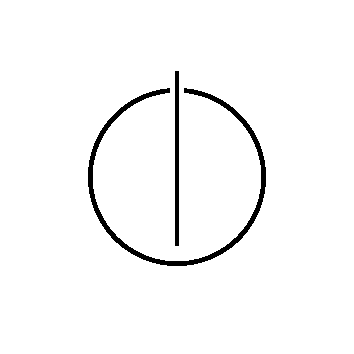
\includegraphics[width=4cm]{InformaticsLogo}
\end{figure}

\end{center}

\thispagestyle{empty}

\vspace{8mm}
\begin{center}
\oTUM{4cm}

\vspace{5mm}     
\huge FAKULT{\"A}T F{\"U}R INFORMATIK\\ 
\vspace{0.5cm}
\large DER TECHNISCHEN UNIVERSIT{\"A}T M{\"U}NCHEN\\
\end{center}

\vspace{5mm}

\begin{center}
{\Large \doctype\ in \faculty}
\vspace{8mm}

\begin{spacing}{1.3}
{\LARGE \title}\\
\vspace{8mm}

{\LARGE \titleGer}\\
\vspace{8mm}
\end{spacing}

\begin{tabular}{ll}
\Large Author:     & \Large \author     \\[2mm]
\Large Supervisor: & \Large \supervisor \\[2mm]				
\Large Advisor:	   & \Large \advisor    \\[2mm]
\Large Date:       & \Large \date
\end{tabular}

\vspace{1mm}

\begin{figure}[hb!]
\centering
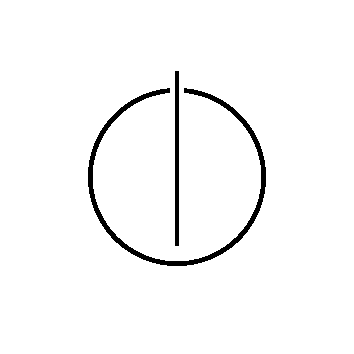
\includegraphics[width=4cm]{InformaticsLogo}
\end{figure}

\end{center}
\newpage
\thispagestyle{empty}
\mbox{}
\clearpage
\thispagestyle{empty}
\vspace*{0.8\textheight}
\noindent
I assure the single handed composition of this master thesis only supported by declared resources,

\vspace{15mm}
\noindent
Munich, \date \hspace{\stretch{1}} \author
\newpage



\newpage
\thispagestyle{empty}
\mbox{}

\chapter*{Acknowledgements}


\pagenumbering{roman}

\selectlanguage{english}
\begin{abstract}

Recent advances in Convolutional Neural Networks (CNN) have been able to conquer Computer Vision tasks and even surpass human performance. CNN algorithms are characteristically data-hungry, and obtaining domain-specific labeled data is often a cumbersome manual resource-heavy task. In this text we explore the use of synthetic data to train a CNN to perform image classification of different fasteners.

\textit{Note:}

\textit{\textbf{1. paragraph:} What is the motivation of your thesis? Why is it interesting from a scientific point of view? Which main problem do you like to solve?}

The motivation for my thesis stems from CNN algorithms' hunger for labeled images in order to train for classification tasks and produce performant results. Obtaining a large corpus of labeled images is a difficult task, especially when we wish to train a network to classify a domain-specific dataset.

\textit{\textbf{2. paragraph:} What is the purpose of the document? What is the main content, the main contribution?}
In this document we explore the use of synthetic images to augment the training data for a given CNN. We explore the power of synthetic data to produce acceptable results while using as little real data as possible. The intuition comes from the ease of rendering a large synthetic dataset on demand.

\textit{\textbf{3. paragraph:} What is your methodology? How do you proceed?}
We explore the ratio of synthetic to real images that can be used for training a CNN and obtain good results.

\end{abstract}

\clearpage

\selectlanguage{german}
\begin{abstract}

%abstract german

\textit{Note: Insert the German translation of the English abstract here.}

\end{abstract}

\clearpage

\selectlanguage{english}


\tableofcontents
\clearpage

\clearpage

\begin{acronym}
\acro{GUI}{Graphical User Interface}

\end{acronym}

\pagenumbering{arabic}

\fancyhead{}
\pagestyle{fancy}
\fancyhead[LE]{\slshape \leftmark}
\fancyhead[RO]{\slshape \rightmark}
\headheight=15pt










%------- CHAPTER 1 -------

\chapter{Introduction}

\textit{Note: Introduce the topic of your thesis, e.g. with a little historical overview.}

\section{Problem}

\textit{Note: Describe the problem that you like to address in your thesis to show the importance of your work. Focus on the negative symptoms of the currently available solution.}

\section{Motivation}

\textit{Note: Motivate scientifically why solving this problem is necessary. What kind of benefits do we have by solving the problem?}

\section{Objectives}

\textit{Note: Describe the research goals and/or research questions and how you address them by summarizing what you want to achieve in your thesis, e.g. developing a system and then evaluating it.}

\section{Outline}

\textit{Note: Describe the outline of your thesis}










%------- CHAPTER 2 -------

\chapter{Background}

\textit{Note: Describe each proven technology / concept shortly that is important to understand your thesis. Point out why it is interesting for your thesis. Make sure to incorporate references to important literature here.}

\section{Supervised Machine Learning}
\subsection{Overview}
\subsection{Image Classification}

\section{Deep Neural Networks}

\section{Convolutional Neural Networks (CNNs)}
\subsection{CNN Building Blocks}
\subsection{CNN Architectures}
\subsubsection{VGG16}
\subsubsection{VGG19}
\subsubsection{Resnet}
\subsubsection{Inception}

\section{Small Mechanical Part Classification}










%------- CHAPTER 3 -------

\chapter{Related Work}

\textit{Note: Describe related work regarding your topic and emphasize your (scientific) contribution in \textbf{contrast} to existing approaches / concepts / workflows. Related work is usually current research by others and you defend yourself against the statement: ``Why is your thesis relevant? The problem was already solved by XYZ.'' If you have multiple related works, use subsections to separate them.}

\section{CNN based Image Classification}
\section{Image Classification using Synthetic Images}










%------- CHAPTER 4 -------

\chapter{Analysis}

%\textit{Note: This chapter follows the Requirements Analysis Document Template in \cite{bruegge2004object}. 
%\textbf{Important:} Make sure that the whole chapter is independent of the chosen technology and development platform. The idea is %that you illustrate concepts, taxonomies and relationships of the application domain independent of the solution domain!
%Cite \cite{bruegge2004object} several times in this chapter.}

\section{Overview}

Our goal is to develop a system that classifies images of different small mechanical parts (SMPs), and to do so as accurately as possible. To realize this goal, we decide to leverage state-of-the-art advancements in Convolutional Neural Network algorithms in the field of computer vision, and more specifically, the sub-field of image classification.

We aim to build a system that scales up well, ie. we would like the classification system to easily adapt new small mechanical parts. Moreover we would like to build a system that can scale up to around 10,000 classes.

CNN algorithms are characteristically data-hungry. The classification accuracy of a CNN algorithm is proportional to the amount of images that are fed in as input. Given the large number of classes, the task of collecting images of each small mechanical part becomes time-consuming and labour-intensive. To combat this problem, we decide to augment the training data of our algorithms with \textit{synthetic images}: 2-dimentional renditions of 3-dimensional computerized graphical models of the small mechanical parts. We hypothesize that our synthetically augmented training set will yield a higher accuracy, whilst minimizing the manual effort needed to take real images of the small mechanical parts.

\section{Requirements}

\subsection{Functional Requirements}

Functional requirements (FRs) describe the interactions between the system and the its environment independent of its implementation. \cite{bruegge2004object}.

The system's main function is to classify images of different small mechanical parts. Furthermore, the system needs to be dynamic and scalable to accomodate new small mechanical parts. To ensure that the system is able to classify images accurately, while leveraging synthetic input images, we introduce the folloing Functional Requirements.

\begin{itemize}
  \item [FR1] \textbf{Generate Synthetic Images}: Given a 3D model of a small mechanical part, the system should generate a set of synthetic images of said model. The system should apply a set of random transformations to the 3D model before rendering the 2D synthetic image to ensure that the generated dataset captures the SMP from as many angles in as many positions as possible.

  \item [FR2] \textbf{Add New Class to Image Classifier}: The system should accomodate the addition of a new SMP to the classifier. This extends to the ability of the system to accomodate for new input training data, and the ability to label a new output class

  \item [FR3] \textbf{Adjust input data split}: The system should allow for changes in the training, validation and testing input data which is assigned as input to the image classifier. This includes changing the number of images in each set and manipulating the ratio of synthetic to real images in the training split.

  \item [FR4] \textbf{Retrain Image Classifier}: The system should be dynamic enough to retrain the image classifier. This step is usually taken after the augmenting or adjustment of the input data split.

  \item [FR5] \textbf{Fine-Tune Image Classifier}: The underlying CNN algorithm should be subject to fine-tuning in order to maximize the accuracy of the system.
\end{itemize}

\subsection{Nonfunctional Requirements}

Nonfunctional Requirements (NFRs) are key system requirements that apply to the system as a whole. To maintain the system's general requirements we define the following nonfunctional requirements.

\begin{itemize}
  \item [NFR1] \textbf{Performance}: A performence requirement is the measure of a quantifiable attribute of our system. In our case we would like to track our system's \textbf{classification accuracy}.\\
  We first specify our system's accuracy for a single class to be the percentage of the given class's testing image split that the image classifier correctly predicts. We consequently define our system's classification accuracy to be the image classifier's average prediction accuracy over each class.

  \item [NFR2] \textbf{Adaptability}: Adaptability is the ability to change the system to deal with additional application domain concepts \cite{bruegge2004object}. Our system needs to be dynamic enough to accomodate for new small mechanical parts that can be later added even after the system has been deployed.
\end{itemize}

\section{System Models}

\subsection{Use Case Model}

Use case models represent the relationship between the user group of a system and the general functions that they can execute. A use case model can reduce the complexity of a system and increase its understandability.

The use case model of our system can be found as figure \ref{fig:UCM}. The main protagonist of our system is the mechanical engineer who is tasked with training the system to classify a set of small mechanical parts.

\begin{figure}[h]
\centering
  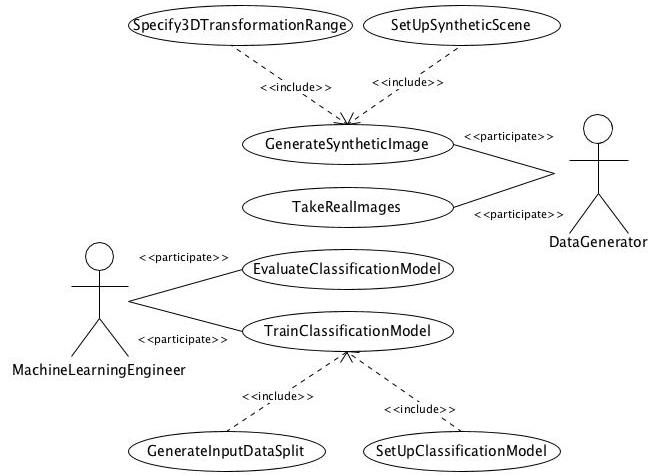
\includegraphics[width=\textwidth]{UCM}
\caption{Use Case Model}
\label{fig:UCM}
\end{figure}

The use case model can be divided into 3 main functions; namely generating synthetic images, obtaining real images, and training an image classifier.

\subsubsection{Generating Synthetic Images}

Generating synthetic images the cornerstone for a synthetically augmented dataset. There's a lot of work that goes into generating the 3D synthetic scene and the corresponding renditions. To increase the understandability of our model, we have separated the the use case that revolve around modeling the SMP 3D model itself as \textit{Specify3DModelTransformations}, and the use case that deals with the synthetic scene environment as \textit{SetUpSyntheticScene}.

\begin{usecase}
  \addtitle{Use Case}{Specify3DModelTransformations}

  \addfield{Participating Actors}{MechanicalEngineer}

  \addscenario{Flow of Events}{
    \item In the modeling software, the MechanicalEngineer chooses the transformations that are applicable to the small mechanical part's 3D model.
    \item For each transformation, the MechanicalEngineer sets the range of each tranformation attribute that will be later used to generate a random position for the synthetic image of the SMP.
  }

  \addfield{Entry Condition}{MechanicalEngineer has modeling software open.}

  \addfield{Exit Condition}{All the desired transformations and their corresponding attributes have been specified.}

  \additemizedfield{Quality Requirements}{
    \item In the effort to achieve the Performance Non-Functional requirement, synthetic images have to look as photo realistic as possible. The 3D transformations should strive to output the range of positions that the respective SMP can be placed in.
  }
\end{usecase}

\begin{usecase}
  \addtitle{Use Case}{SetUpSyntheticScene}

  \addfield{Participating Actors}{MechanicalEngineer}

  \addscenario{Flow of Events}{
    \item In the modeling software, the MechanicalEngineer places the 3D model of the SMP on a horizontal plane as if lying on a table.
    \item The MechanicalEngineer sets the background of the horizontal plane to mimic the background of the real images in the dataset.
    \item The MechanicalEngineer sets the lighting condition of the scene to reflect the lighting condition of the environment where the real SMP images are taken.
  }

  \addfield{Entry Condition}{MechanicalEngineer has modeling software open.}

  \addfield{Exit Condition}{In the modeling software, the 3D model of the SMP should be lying on a horizontal plane with a background and lighting condition that reflect the environment of the real SMP images.}

  \additemizedfield{Quality Requirements}{
    \item The synthetic scene should look as photorealistic as possible. This helps the Image Classifier achieve a higher classification accuracy using the synthetic images.
  }
\end{usecase}

\begin{usecase}
  \addtitle{Use Case}{GenerateSyntheticImages}

  \addfield{Participating Actors}{MechanicalEngineer}

  \addscenario{Flow of Events}{
    \item The MechanicalEngineer specifies the desired number of output synthetic images.
    \item The modeling software generates the desired number of output synthetic images. Each image is a rendition of the scene after the transformations have been applied to the 3D model.
  }

  \addfield{Entry Condition}{MechanicalEngineer has modeling software open.}

  \addfield{Exit Condition}{The MechanicalEngineer obtains a set of synthetic images for the specified SMP that can be later used to train the Image Classifier.}
\end{usecase}

\subsubsection{Obtaining Real Images}

\begin{usecase}
  \addtitle{Use Case}{TakeRealImages}

  \addfield{Participating Actors}{MechanicalEngineer}

  \addscenario{Flow of Events}{
    \item The MechanicalEngineer places the camera over a plane.
    \item The MechanicalEngineer sets the SMP over the plane in a random position, such that the full SMP body is within the viewfield of the camera.
    \item The MechanicalEngineer takes a picture of the SMP.
    \item The MechanicalEngineer repeats steps 2 and 3 until the desired number of real images of the SMP is reached.
    \item The MechanicalEngineer resizes the images to correspond to the input image size of the Image Classifier. 
  }

  \addfield{Entry Condition}{}

  \addfield{Exit Condition}{The MechanicalEngineer obtains a set of real images for the specified SMP that can be later used to train the Image Classifier.}

  \additemizedfield{Quality Requirements}{
    \item The lighting of the environment should eliminate shadows and light reflections on the SMP surface.
  }
\end{usecase}

\subsubsection{Training the Image Classifier}

Training the image classifier requires some underlying work. We have chosen to model this use case as one that includes setting up the input data and configuring the image classifier (modeled as \textit{SetInputDataSplit} and \textit{SetUpImageClassifier} respectively).

\begin{usecase}
  \addtitle{Use Case}{TrainImageClassifier}

  \addfield{Participating Actors}{MechanicalEngineer}

  \addscenario{Flow of Events}{
    \item The MechanicalEngineer configures the dataset structure: number of images for training, validation and testing, as well as the ratio of real to synthetic images in the training split.
    \item The MechanicalEngineer chooses a convolutional neural network architecture for the Image Classifier.
    \item The MechanicalEngineer fine-tunes the CNN by manipulating its hyperparameters.
  }

  \addfield{Entry Condition}{For each SMP set to be classified by the Image Classifier, the corresponding real and synthetic images should be generated and ready for use.}

  \addfield{Exit Condition}{The Image Classifier outputs the maximum possible accuracy given the input dataset.}
\end{usecase}

\subsection{Analysis Object Model}

The analysis object model is a visual dictionary of the main concepts visible to the user \cite{bruegge2004object}. The analysis object model depicts a system's entites, their corresponding attributes and functions, and illustrates the relationship between said entitie. Figure \ref{fig:AOM} represents the analysis object model of our system.

\begin{figure}[h]
\centering
  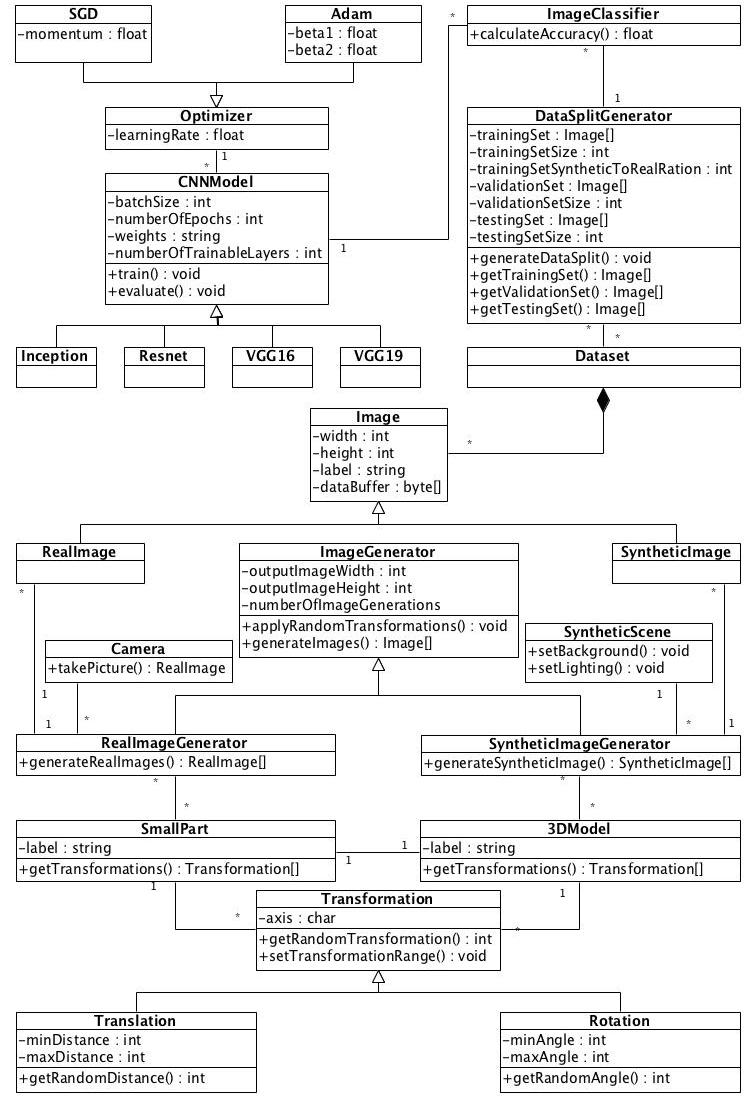
\includegraphics[width=\textwidth]{AOM}
\caption{Analysis Object Model}
\label{fig:AOM}
\end{figure}

\subsubsection{SmallMechanicalPart}
A small mechanical part is the main subject of our system. It is an object that our system aims to classify. Each SMP has a unique identifying label string.

\subsubsection{3DModel}
A 3DModel of a small mechanical part is the graphical model which helps our system create synthetic images. Each SMP has a corresponding 3DModel. Each 3DModel has the same label as its SMP counterpart.

\subsubsection{Transformation}
Each SMP and 3DModel have a list of applicable transformations. A transformation is executed on an axis (x, y or z), and can either be a Translation or a Rotation.
At image generation time, each transformation outputs a random value between its defined maximum and minimum. We define a range to limit an object's transformation. For instance, we don't want to translate an SMP so far as to remove it from the camera's viewfield.

\subsubsection{ImageGenerator}
ImageGenerator is the class that does the heavy lifting when it comes to creating images. It applies the random transformations on the target object and generates an image with a specified width and height.
ImageGenerator is an abstraction of 2 classes. SyntheticImageGenerator is responsible for applying the transformations on 3Dmodels and generating SyntheticImages, while RealImageGenerator uses a camera to take pictures of small mechanical objects and output their corresponding RealImages.

\subsubsection{Image}
Image is a generalization of RealImage and SyntheticImage. Image stores information like width, height and label of the image. Moreover it contains a dataBuffer which contains the actual image pixel values.

\subsubsection{Dataset}
Dataset is a composition of Images. It is the image repository which is used by the ImageClassifier for training and evaluation.

\subsubsection{DataSplitGenerator}
DataSplitGenerator splits the Dataset into a training set, validation set and testing set. This split prepares the data for consumption by the ImageClassifier.

\subsubsection{CNNModel}
CNNModel is the convolutional neural network algorithm that is trained for image classification. CNNModel is an abstraction of 4 different CNN architectures, namely Inception, Resnet, VGG16 and VGG19. Furthermore, CNNModel defines the weights that are used to initialize the CNN to leverage the power of transfer learning. CNNModel also sets the number of trainable layers in a network to potentially preserve the initial weights and speed up training.

\subsubsection{Optimizer}
Each CNNModel has an Optimizer. An Optimizer is the function aims to close the gap between the model's predictions of the validation set labels and their corresponding ground truth. The Optimizer operates in the CNNModel's training phase. Optimizer is an abstraction of 2 different optimizers that we use in our system. Specifically SGD (Stochastic Gradient Descent), and Adam.

\subsubsection{ImageClassifier}
ImageClassifier orchestrates the feeding of data into the CNNModel for training. Moreover, it uses the testing set to calculate the accuracy of the trained model.


\subsection{Dynamic Model}

The dynamic model is focused on the behavior of the system. Sequence diagrams, activity diagrams and state machines are usually used to depict dynamic models \cite{bruegge2004object}. In this section we present 2 activity diagrams that depict the 2 main workflows of our system.

\subsubsection{Dataset Generation}

Figure \ref{fig:AD1} depicts the workflow of activities required to generate a dataset. The MechanicalEngineer selects a small mechanical part and its corresponding 3D model. The MechanicalEngineer then proceeds to generate the real and synthetic images. Finally the images are combined to form a dataset.

\begin{figure}[h]
\centering
  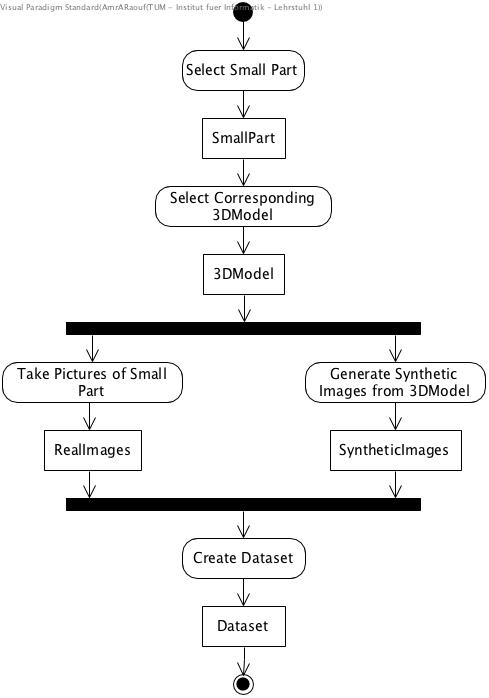
\includegraphics[width=\textwidth]{AD1}
\caption{Activity Diagram depicting the workflow required for Dataset generation}
\label{fig:AD1}
\end{figure}

\subsubsection{Training the Image Classifier}

Figure \ref{fig:AD2} describes the workflow of activities required to train the image classifier. The MechanicalEngineer splits the data into training, validation and testing sets. The MechanicalEngineer then creates a CNN model. Next the MechanicalEngineer feeds the training data to the CNN model to obtained a trained CNN model. The MechanicalEngineer then evaluates the trained CNN model accuracy using the testing set. If the accuracy of the trained CNN model is not sufficient, the CNN model is fine tuned and re-trained.

\begin{figure}[h]
\centering
  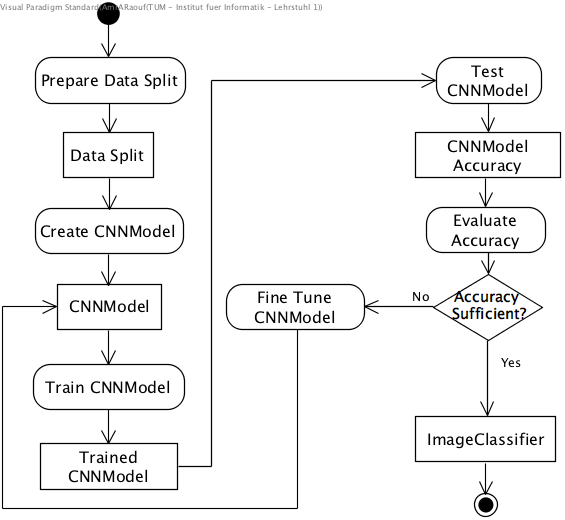
\includegraphics[width=\textwidth]{AD2}
\caption{Activity Diagram describing the workflow required to train the Image Classifier}
\label{fig:AD2}
\end{figure}









%------- CHAPTER 5 -------

\chapter{System design}

\textit{Note: This chapter follows the System Design Document Template in \cite{bruegge2004object}. 
You describe in this chapter how you map the concepts of the application domain to the solution domain. Some sections are optional, if they do not apply to your problem.
Cite \cite{bruegge2004object} several times in this chapter.}

\section{Overview}

\textit{Note: Provide a brief overview of the software architecture and references to other chapters (e.g. requirements analysis), references to existing systems, constraints impacting the software architecture.}

\section{Design Goals}

\textit{Note: Derive design goals from your nonfunctional requirements, prioritize them (as they might conflict with each other) and describe the rationale of your prioritization. Any trade-offs between design goals (e.g., build vs. buy, memory space vs. response time),
and the rationale behind the specific solution should be described in this section}

\section{Subsystem Decomposition}

\textit{Note: Describe the architecture of your system by decomposing it into subsystems and the services provided by each subsystem. Use UML class diagrams including packages / components for each subsystem.}

\section{Hardware Software Mapping}

\textit{Note: This section describes how the subsystems are mapped onto existing hardware and software components. The description is accompanied by a UML deployment diagram. The existing components are often off-the-shelf components. If the components are distributed on different nodes, the network infrastructure and the protocols are also described.}

\section{Persistent Data Management}

\textit{Note: Optional section that describes how data is saved over the lifetime of the system and which data. Usually this is either done by saving data in structured files or in databases. If this is applicable for the thesis, describe the approach for persisting data here and show a UML class diagram how the entity objects are mapped to persistent storage.
It contains a rationale of the selected storage scheme, file system or database, a description of the selected database and database administration issues.}

\section{Access Control}

\textit{Note: Optional section describing the access control and security issues based on the nonfunctional requirements in the requirements analysis. It also describes the implementation of the access matrix based on capabilities or access control lists, the selection of  authentication mechanisms and the use of encryption algorithms.}

\section{Global Software Control}

\textit{Note: Optional section describing describing the control flow of the system, in particular, whether a monolithic, event-driven control flow or concurrent processes have been selected, how requests are initiated and specific synchronization issues}


\section{Boundary Conditions}

\textit{Note: Optional section describing the use cases how to start up the separate components of the system, how to shut them down, and what to do if a component or the system fails.}










%------- CHAPTER 6 -------

\chapter{Case Study / Evaluation}

\textit{Note: If you did an evaluation / case study, describe it here.}

\section{Design}

\textit{Note: Describe the design / methodology of the evaluation and why you did it like that. E.g. what kind of evaluation have you done (e.g. questionnaire, personal interviews, simulation, quantitative analysis of metrics, what kind of participants, what kind of questions, what was the procedure?}

\section{Objectives}

\textit{Note: Derive concrete objectives / hypotheses for this evaluation from the general ones in the introduction.}

\section{Results}

\textit{Note: Summarize the most interesting results of your evaluation (without interpretation). Additional results can be put into the appendix.}

\section{Findings}

\textit{Note: Interpret the results and conclude interesting findings}

\section{Discussion}

\textit{Note: Discuss the findings in more detail and also review possible disadvantages that you found}

\section{Limitations}

\textit{Note: Describe limitations and threats to validity of your evaluation, e.g. reliability, generalizability, selection bias, researcher bias}











%------- CHAPTER 7 -------

\chapter{Summary}

\textit{Note: This chapter includes the status of your thesis, a conclusion and an outlook about future work.}

\section{Status}

\textit{Note: Describe honestly the achieved goals (e.g. the well implemented and tested use cases) and the open goals here. if you only have achieved goals, you did something wrong in your analysis.}

\subsection{Realized Goals}

\textit{Note: Summarize the achieved goals by repeating the realized requirements or use cases stating how you realized them.}

\subsection{Open Goals}

\textit{Note: Summarize the open goals by repeating the open requirements or use cases and explaining why you were not able to achieve them. \textbf{Important:} It might be suspicious, if you do not have open goals. This usually indicates that you did not thoroughly analyze your problems.}

\section{Conclusion}

\textit{Note: Recap shortly which problem you solved in your thesis and discuss your \textbf{contributions} here.}

\section{Future Work}

\textit{Note: Tell us the next steps  (that you would do if you have more time. be creative, visionary and open-minded here.}



\appendix

\chapter{e.g. Questionnaire}

\textit{Note: If you have large models, additional evaluation data like questionnaires or non summarized results, put them into the appendix.}


\clearpage

\listoffigures
\clearpage

\listoftables
\clearpage

\bibliography{thesis}
\bibliographystyle{alpha}

\end{document}
